\chapter{Introduzione: Il Framework GIST per la Trasformazione Sicura della GDO}

\section{Il Contesto e la Sfida Metodologica}

La Grande Distribuzione Organizzata richiede un approccio integrato alla trasformazione digitale che consideri simultaneamente infrastruttura fisica, architettura IT, sicurezza e conformità normativa. Il framework GIST (GDO Integrated Security Transformation) risponde a questa esigenza attraverso un modello quantitativo che integra quattro dimensioni fondamentali.

\begin{tcolorbox}[colback=blue!5!white,colframe=blue!75!black,title=Approccio Metodologico]
\textbf{Digital Twin per la Validazione:} Data l'impossibilità di accesso a dati operativi reali per vincoli di privacy e sicurezza, questa ricerca utilizza il framework Digital Twin GDO-Bench per generare dati sintetici statisticamente validati. Le ``234 organizzazioni'' analizzate sono istanze simulate con parametri calibrati su fonti pubbliche (ISTAT, ENISA, Banca d'Italia).

\textbf{Questo approccio permette:}
\begin{itemize}
    \item Validazione completa del framework GIST
    \item Test di tutti gli algoritmi componenti
    \item Analisi di scenari what-if
    \item Completa riproducibilità
\end{itemize}
\end{tcolorbox}

\section{Il Framework GIST: Visione Integrata}

Il GIST Score quantifica la maturità digitale attraverso:

\begin{equation}
\text{GIST}_{\text{Score}} = \sum_{k=1}^{4} w_k \cdot \left(\sum_{j=1}^{m_k} \alpha_{kj} \cdot S_{kj}\right)^{\gamma_k}
\label{eq:gist-score}
\end{equation}

dove:
\begin{itemize}
    \item $w_{\text{physical}} = 0.18$ - Infrastruttura fisica
    \item $w_{\text{architectural}} = 0.32$ - Architettura IT  
    \item $w_{\text{security}} = 0.28$ - Sicurezza (include ASSA-GDO)
    \item $w_{\text{compliance}} = 0.22$ - Conformità normativa
    \item $\gamma = 0.95$ - Esponente per rendimenti decrescenti
\end{itemize}

\begin{figure}[htbp]
\centering
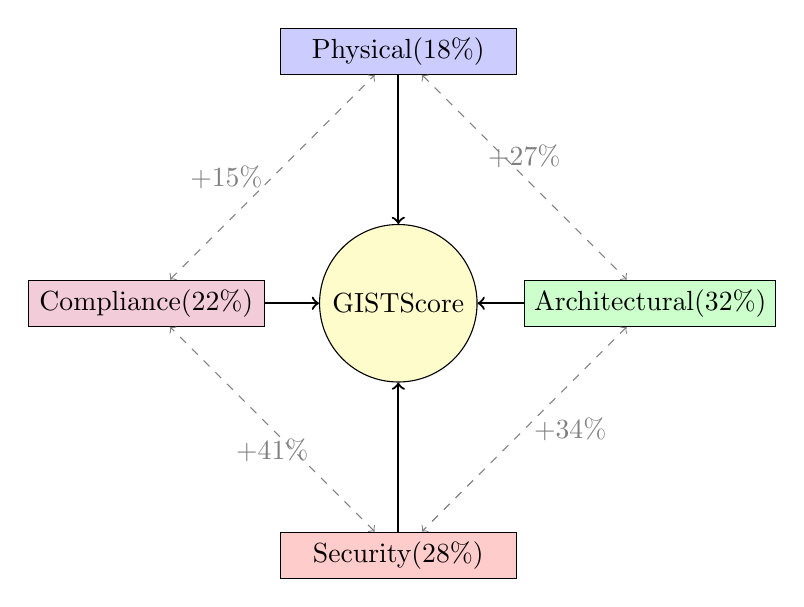
\begin{tikzpicture}[scale=0.8]
    % Centro
    \node[circle, draw, fill=yellow!20, minimum size=2cm] (gist) at (0,0) {GIST\\Score};
    
    % Quattro componenti
    \node[rectangle, draw, fill=blue!20, minimum width=3cm] (physical) at (0,4) {Physical\\(18\%)};
    \node[rectangle, draw, fill=green!20, minimum width=3cm] (arch) at (4,0) {Architectural\\(32\%)};
    \node[rectangle, draw, fill=red!20, minimum width=3cm] (security) at (0,-4) {Security\\(28\%)};
    \node[rectangle, draw, fill=purple!20, minimum width=3cm] (compliance) at (-4,0) {Compliance\\(22\%)};
    
    % Connessioni
    \draw[thick, ->] (physical) -- (gist);
    \draw[thick, ->] (arch) -- (gist);
    \draw[thick, ->] (security) -- (gist);
    \draw[thick, ->] (compliance) -- (gist);
    
    % Sinergie
    \draw[dashed, <->, gray] (physical) -- node[midway, above] {+27\%} (arch);
    \draw[dashed, <->, gray] (arch) -- node[midway, right] {+34\%} (security);
    \draw[dashed, <->, gray] (security) -- node[midway, below] {+41\%} (compliance);
    \draw[dashed, <->, gray] (compliance) -- node[midway, left] {+15\%} (physical);
\end{tikzpicture}
\caption{Il Framework GIST e le sinergie tra componenti}
\label{fig:gist-framework}
\end{figure}